\documentclass[
    margin=1in,
    innermargin=-4.5in,
    ]{tikzposter}

% Choose size here
\geometry{paperwidth=33.11in,paperheight=46.81in} %A0
% \geometry{paperheight=33.11in,paperwidth=23.4in} %A1
    
\usepackage[utf8]{inputenc}
\usepackage{csquotes}
\usepackage{amsmath}
\usepackage{amsfonts}
\usepackage{amsthm}
\usepackage{amssymb}
\usepackage{mathrsfs}
\usepackage{graphicx}
\usepackage{lipsum}
\usepackage[export]{adjustbox}
\usepackage{tcolorbox}
\usepackage[font=small,labelfont=bf]{caption} % Required for specifying captions to tables and figures
\usepackage{enumitem}
%\usepackage[backend=biber,style=numeric]{biblatex}
\usepackage[style=authoryear,backend=biber,
            natbib=true,maxcitenames=1]{biblatex}
\usepackage{glasgow-poster-theme}
\makeatletter
\setlength{\TP@visibletextwidth}{31.0in}
\setlength{ \TP@visibletextheight}{45in}
\makeatother
\usepackage{bm}
\usepackage{bbm}

\addbibresource{references.bib}

% set theme parameters
\tikzposterlatexaffectionproofoff
\usetheme{UniGlasgowTheme}
\usecolorstyle{UniGlasgowStyle}

\usepackage[scaled]{helvet}
\renewcommand\familydefault{\sfdefault} 
\renewcommand{\vec}[1]{\bm{#1}}
\newcommand{\Tr}{\text{Tr}}
\usepackage[T1]{fontenc}

% Adjust trim if title doesn't have two lines
\titlegraphic{
\includegraphics[width=0.35\linewidth, trim={0 -2cm 0 0cm}, clip]{figures/logo_glasgow.jpg}}

\title{\parbox{0.8\linewidth}{\textbf{Can the Detection of Roman}\\ \textbf{Roads be Automated with the}\\ \textbf{Application of GeoAI?}}}
\author{Ian Turton\textsuperscript{1}}
\institute{\textsuperscript{1}School of Geographical and Earth Sciences, University of Glasgow}



% begin document
\begin{document}
\maketitle
\centering
\begin{columns}
    \column{0.5}
    \block{Introduction}{
       In the past decade there has been an increased reporting of the use LiDAR data in the discovery of archaeological features in the landscape mainly driven by the increased availability of this type of data as a by-product of flood prevention or forest surveys \citep{stular_visualization_2012, rostain_two_2024}. Examples from Britain include \citeauthor{gethin_roman_2014} (\citeyear{gethin_roman_2014}) discovering a Roman marching camp and road fragment in North Wales using LiDAR data provided by the Environment Agency, and \citet{small_lost_2016} combines the LiDAR data with other sources to show the route of a Roman road in Southern England. Recently \citet{parcero-oubina_remote_2023} have presented their work on the detection of some previously undiscovered Roman roads in the SW of England using a combination of least cost paths between known Roman occupation locations and then verifying these paths by examining the recently released Environment Agency LiDAR data. \citet{lewis_probabilistic_2021} has shown a similar process but compares the findings of the model to a known Roman road (High Street) in an attempt to discover the effects of error in the height calculated in the DTM derived from the LiDAR measurements. 

However, in all of these cases the interpretation and discovery was carried out by a trained archaeologist looking at the LiDAR data set (in a variety of representations) and often by combining it with other information, including the known location of other roman artefacts. There is now 1m resolution LiDAR data available for the whole of Great Britain and in many places 50cm resolution data is available freely to researchers (and the general public). There is clearly more data than any one researcher (or even a research group) to investigate closely. This is a data rich problem that is ripe for the introduction of artificial intelligence (AI) or machine learning technology (ML) to winnow the grain from the chaff. \citet{abriha_strategies_2023} look at the use of AI technologies to the discovery of buildings from remote sensed imagery. \citet{albrecht_learning_2019} present the development of a artificial neural network based workflow to detect archaeological features in large LiDAR data.}
    
    \block{Method}{
        \begin{center}
            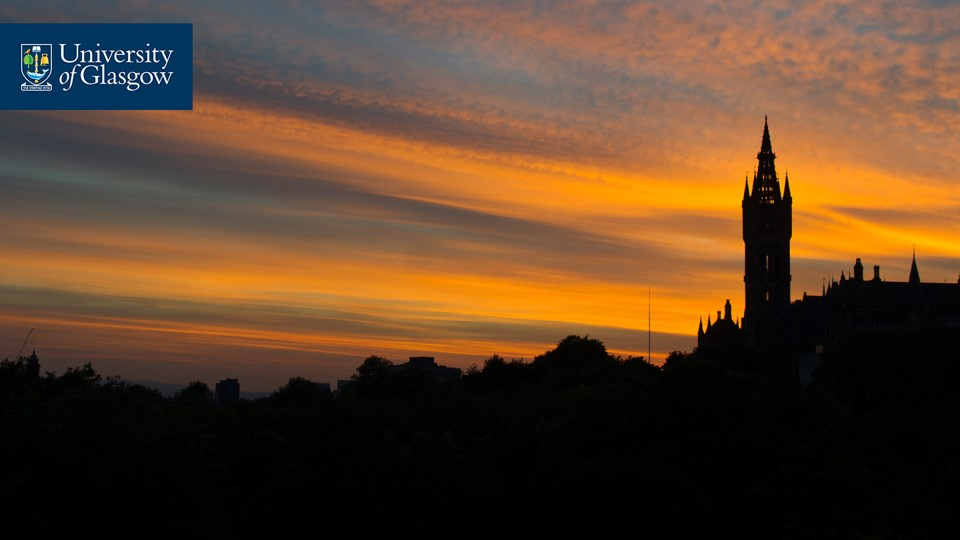
\includegraphics[width=0.8\linewidth]{figures/glasgow_sunset.jpg}
            \captionof{figure}{Sunset in Glasgow}
        \end{center}
        
        \vspace{1cm}
    
        \lipsum[100]
        \lipsum[100]
        \lipsum[100]
    }


    \column{0.5}
    

    \block{Conclusions}{
        \lipsum[100]
      
    }
    
    \block{References}{
                \begin{center}
                   \mbox{}\vspace{-1\baselineskip}
    \printbibliography[heading=none] 
        \end{center}
        }

    \block{Acknowledgements}{The author acknowledges the support from the UK Research and Innovation Future Leaders Fellowships ``Missing Data as Useful Data'', grant number MR/Y011856/1, ``Indicative Data: Extracting 3D Models of Cities from Unavailability and Degradation of Global Navigation Satellite Systems (GNSS)'', grant number MR/S01795X/2, and the Alan Turing Institute-DSO partnership project on ``Multi-Lingual and Multi-Modal Location Information Extraction''}

\end{columns}
\end{document}